\chapter{Iterative development}\label{chapter:prototype}

% Shirley et al. : human-centered design process
%This iterative process can be human-centered design process described in \cite{shirley:2009}.

This chapter describes how the idea presented in chapter \ref{chapter:literature_study} is tested and improved through different development cycles. First the evaluation and development techniques used for the tests are described.


\section{Methodology}\label{chapter:prototype:section:methodology}

\subsection{Prototyping}\label{chapter:prototype:section:methodology:subsection:development}

% rapid prototyping

There are three types of prototypes that were used in the iterations:

\begin{itemize}
	\item Paper prototype;
	\item Digital prototype with 'fake' data or interaction effects;
	\item Digital prototype with working implementation.
\end{itemize}

It is obvious that for each category the resources that are required to build the prototype differ. The objective is to filter out most of the issues in the low cost designs, avoiding a greater cost in the more expensive prototypes.

\emph{Paper prototyping}\index{paper prototyping} is defined as "a variation of usability testing where representative users perform realistic tasks by interacting with a paper version of the interface that is manipulated by a person 'playing computer', who doesn’t explain how the interface is intended to work"\cite{snyder:2003:web}. It is a technique for designing, testing, and refining user interfaces \cite{snyder:2003}, and is closely related to usability testing \cite{snyder:2003:web}. In the last decade it has become a regularly applied technique in major businesses such as IBM, Digital, Honeywell, and Microsoft among others\cite{snyder:2003}.

Digital prototypes capture a portion of the functionality in an application. In the early stages of the design process, this application usually works with static data, or a limited number of screen transitions. This allows for more flexibility when certain functionality has to be altered. In later iterations the static data is replaced with real data. In such prototypes, the effects of performance of algorithms and interface responsiveness can be analyzed in greater detail.


\subsection{Evaluation techniques}\label{chapter:prototype:section:methodology:subsection:evaluation}

The evaluation of an application prototype can be performed using one or more different techniques, and based on a range of varying criteria, such as: usability, usefulness, meaning, efficiency, accuracy and so on. Various techniques exist, such as questionnaires, usability engineering, expert evaluation, and usage tracking\cite{duval:2012:chi:evaluation}.

Methods may be \emph{formative}\index{formative!evaluation technique} or \emph{summative}\index{summative!evaluation technique}. Formative means that the evaluation occurs simultaneously with user task execution. Summative occurs after the user has performed all the required tasks\cite{duval:2012:chi:evaluation}.

The explanation system will be evaluated based on seven aims described by Tintarev and Masthoff \cite{tintarev:2007:SER:1547550.1547664} listed in table \ref{table:explanation:aims}. Also learnability and memorability, properties of usability as described by Nielsen\cite{nielsen:1993:UE:529793}, are also evaluated. An insight evaluation method developed by Chris North \cite{north:2006} is used to measure transparency, as described in section \ref{chapter:literature_study:section:user:subsection:insight}. Usability evaluation methods are used to measure satisfaction, efficiency, learnability and memorability. Trust, effectiveness, and persuasiveness are also evaluated during the user study. Scrutability is not supported by the explanation system.

Both usability and insight gaining methods are a variation on \emph{usability engineering}\index{usability engineering} called \emph{think aloud}\index{think aloud} user tests. Additionally, a type of questionnaires called \emph{system usability scale} (SUS)\index{system usability scale} \emph{questionnaires}\index{questionnaire} are used to obtain a quantification of the perceived usability by test users, in terms of perceived learnability and satisfaction. Such a quantification may allow us to identify positive or negative trends in the usability throughout the iterations.

In order to perform reliable usability tests, the test users have to be representative for the actual user population\cite{duval:2012:chi:evaluation, north:2006}. The tasks that are being used, have to be representative of the system usage. Tasks also have to correspond to research questions to obtain relevant results\cite{snyder:2003}.

The number of users can often be limited. As the number of detectable problems is likely to be finite, from a certain point on testing more users will not produce new or better results\cite{duval:2012:chi:evaluation, nielsen:2012:nngroup:diminishing_returns}. The graph in figure \ref{fig:nielsengraph}, adapted from \cite{nielsen:2012:nngroup:diminishing_returns}, illustrates this phenomenon.

Nielsen argues that as a rule of tumb, five test users is enough to acquire reliable and valuable test results. Instead of doing one test with 15 users, use three iterations with 5 users each. Based on the graph, the first iteration will discover the majority of the usability problems; the next two tests will uncover the remaining 15\% of issues. Of course, this only holds on the condition that tasks performed by the users are similar for each iteration. Between each iteration, corrections are applied to the design\cite{nielsen:2012:nngroup:diminishing_returns}. Between these groups of tests, detected usability problems are addressed, and hopefully resolved which can be verified in the next iteration.

\begin{figure}
	\begin{center}
		\includegraphics[width=250px]{img/nielsen2012_usertests}
	\end{center}
	\caption{The curve shows the user test's diminishing returns beyond a certain amount of test users; adapted from \cite{nielsen:2012:nngroup:diminishing_returns}.}
	\label{fig:nielsengraph}
\end{figure}


\subsubsection{Usability engineering}

In \cite{duval:2012:chi:evaluation}, two methods are described to perform usability engineering tests: usability labs, and think aloud\index{think aloud} testing. In a usability lab the user is observed while performing certain tasks. Data on task completion time, mouse clicks, eye-movement can be collected. Direct observation or cameras can be used to observe the user. To mimic real-life situations, also complete settings can be recreated in which the users would normally use the application\cite{duval:2012:chi:evaluation}.

Using usability labs can be rather costly, since labs need to be available and the required equipment may be expensive. The think aloud protocol is a variation on the usability lab method and is cheaper to perform, cf. 'discount usability engineering'\cite{duval:2012:chi:evaluation}. During a think aloud test, the user describes his/her reasoning for each action he/she undertakes\cite{nielsen:2012:nngroup:think_aloud}. This method has several advantages and disadvantages, as listed in table \ref{table:usability_engineering}, based on \cite{nielsen:2012:nngroup:think_aloud} and \cite{snyder:2003}.


\begin{table}%
	\begin{center}
		\begin{tabular}{l p{300px}}
			\hline
			Advantages		&		It is cheap to perform; \\
										&		It is robust; \\
										&		It is flexible; \\ % giving required freedom to perform insight tests
										&		It is convincing; \\
										&		It is easy to learn; \\
			\hline
			Disadvantages	&		It creates an unnatural situation, as users usually don't say out loud everything they are about to do or think; \\
										&		The user may tend to filter his/her statements to avoid saying things that he/she may find silly or uninteresting; \\
										&		The facilitator may introduce bias in user behavior if he/she provides too much information when answering or instructing users; \\
			\hline
		\end{tabular}
	\end{center}
	\caption{Advantages and disadvantages of the think aloud protocol.}
	\label{table:usability_engineering}
\end{table}

\subsubsection{Questionnaires}

To obtain information other than observational data, the user is presented with a summative questionnaire. Questionnaires are used to obtain subjective information from the user about the user's experiences. Table \ref{table:questionnaires} lists several advantages and disadvantages of the use of questionnaires in usability studies, based on \cite{kirakowski:2013}.

\begin{table}%
	\begin{center}
		\begin{tabular}{l p{300px}}
			\hline
			Advantages		&		Evaluates the point of view of the user; \\
										&		Measures gained from a questionnaire are to a large extent, independent of the system, users, or tasks to which the questionnaire was applied; \\
										&		Quick and cost effective; \\
			\hline
			Disadvantages	&		Only the user's reaction as the user perceives the situation; \\
										&		Lack of detail, as questionnaires are usually designed to fit a number of different situations; \\
										&		Subjective data must be enhanced with performance, mental effort, and effectiveness data. \\
			\hline
		\end{tabular}
	\end{center}
	\caption{Advantages and disadvantages of the questionnaires.}
	\label{table:questionnaires}
\end{table}


There are several standardized questionnaires. The one used for the application evaluation is the system usability scale\index{system usability scale} (SUS). A system usability scale test is a questionnaire that consists out of ten specific questions that attempts to measure the user's perception of the application's usability. Each question is answered by checking one out of five checkboxes: checkbox one corresponds to strong disagreement with the statement, the fifth checkbox corresponds to strong agreement with the statement\cite{sauro:2011}. The ten questions are listed in table \ref{table:sus_questions}.

To interpret SUS results, the scores should be compared on a percentile rank. Figure \ref{figure:sus_percentile} shows a graph by Jeff Sauro adapted from \cite{sauro:2011}. A SUS score of 80 means then that the perceived usability is higher than almost 90 percent of the products tested in Sauro's user studies.

\begin{figure}%
	\begin{center}
		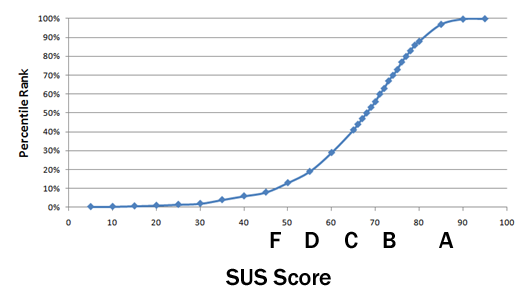
\includegraphics[width=280px]{img/sus_curve}%
	\end{center}
	% http://www.measuringusability.com/sus.php
	\caption{Percentile ranks associate with SUS scores and letter grades, adapted from \cite{sauro:2011}.}%
	\label{figure:sus_percentile}%
\end{figure}


\section{Iterations}

We will now give an overview of the setup for the user studies. In the next subsections we will discuss each iteration in more detail.

To increase domain relevance, it is important to have representative test users. The participants were selected from the campus and among acquaintances and were between $21$ and $27$ years of age. For all of the iterations combined, a total of $15$ users participated in the user study of whom $12$ were male and $3$ were female. Based on the categorization in table \ref{table:jennings:listeners}, $5$ users identied themselves as \emph{savants}, $7$ as \emph{enthousiasts}, and $3$ as \emph{casuals}. Although they had a notion of what a recommender system was, none of them knew how recommendation algorithms worked.

The test users were spread among four different iterations. Some of the users took part in multiple tests. The distribution of users can be seen in table \ref{table:evaluation:users}. There are two particular incentives to let users participate in more than one test:

\begin{enumerate}
	\item These users can provide direct feedback on changes made between the iterations that addressed certain usability issues.
	\item As insight builds up over time, it would be interesting to go beyond the scope of a single user test that only lasts $30$ to $60$ minutes. If given the opportunity, users may develop new ways to apply their previously obtained insights, amplifying its deep, serendipitous, complex and qualitative aspects.
\end{enumerate}

\begin{table}
	\caption{The distribution of test users used in the evaluations for each iteration.}
	\begin{center}
		\begin{tabular}{l | l l l l }
				\hline
																	& \multicolumn{4}{c}{\textbf{Iteration}} \\
																\cline{2-5}
																& $1$ & $2$ & $3$ & $4$ \\
			\hline
			Number of users						&	5 	&	5		&	5		&	10	\\
			From previous iterations	&	-  	&	2 	&	3		&	5	\\
			\hline
		\end{tabular}
	\end{center}
	\label{table:evaluation:users}
\end{table}

Over the four iterations the application was incrementally improved. Table \ref{table:iteration:aims} gives an overview of which aims were evaluated for the prototype in each iteration. The reason why trust, effectiveness, and persuasion are only tested in the last iteration, was that in iteration $1$ and $2$ no data from the active user was processed. As a result, it would be rather pointless to test for effectiveness if the user profile does not correspond to the active user's taste. In iteration three, we focus mainly on usability aspects.

\begin{table}
	\caption{The explanation aims that were evaluated in each iteration.}
	\begin{center}
		\begin{tabular}{l | l l l l }
			\hline
			\textbf{Aim} 							& \multicolumn{4}{c}{\textbf{Iteration}} \\
																\cline{2-5}
																& $1$ & $2$ & $3$ & $4$ \\
			\hline
			Tra. Sat., Efc., Learn.		&	x 	&	x		&	x		&	x	\\
			Mem.											&	  	&	x		&	x		&	x	\\
			Trust, Efk., Pers.				&	  	&	 		&	 		&	x	\\
			\hline
		\end{tabular}
	\end{center}
	\label{table:iteration:aims}
\end{table}



%%%%%%% ITERATION 1
\subsection{Iteration 1: paper prototype}\label{chapter:prototype:section:paper}

% 6. testen...
%		+ doel: wat wil je te weten komen?
%		+ methode: hoe ga je dat te weten komen?
%		+ rationale: welke andere manieren heb je overwogen en waarom niet weerhouden?
%		+ wie, wat, waar: n, demographics, logistics, ...
%		+ resultaten: wat heb je gemeten, geobserveerd? (zonder interpretatie)
%		+ besluit: wat ben je te weten gekomen? (link naar resultaten)
% 7. itereren...
%		+ doel: belangrijkste proble(e)m(en) dat/die je wil aanpakken
%		+ alternatieven: hoe kan je problemen aanpakken
%		+ keuze: en rationale
%		+ herneem die problemen bij volgende iteratie!

\subsubsection{The prototype}\label{chapter:prototype:section:paper:prototype}

The paper prototype that was tested, consisted out of a single screen. On this screen a visualization was drawn by hand. A number of copies were made of this drawing and by changing certain parts of the visualization, transitions within the visualization could be mimicked as users interacted with the screen. A selection of these screens are shown in figure \ref{figure:paper_prototype}.

% BEGIN FIGURE : paper prototype
\begin{figure}
	\centering
	\begin{subfigure}[t]{0.3\textwidth}
					\centering
					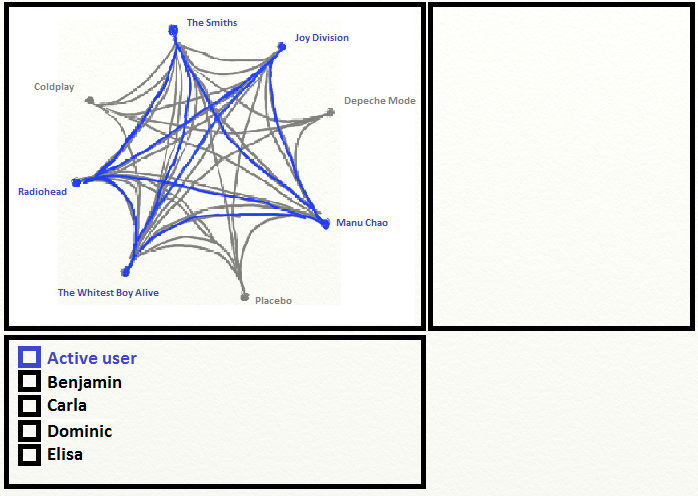
\includegraphics[width=\textwidth]{img/paper_prototype_default}
					\caption{The default visualization with the active users items highlighted.}
					\label{figure:paper_prototype_default}
	\end{subfigure}%
	~
	\begin{subfigure}[t]{0.3\textwidth}
					\centering
					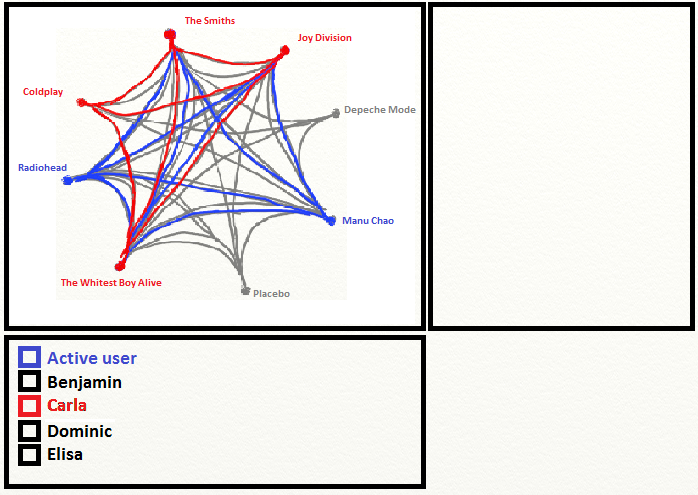
\includegraphics[width=\textwidth]{img/paper_prototype_user_click}
					\caption{Clicking/hovering a user list element.}
					\label{figure:paper_prototype_user_click}
	\end{subfigure}
	~
	\begin{subfigure}[t]{0.3\textwidth}
					\centering
					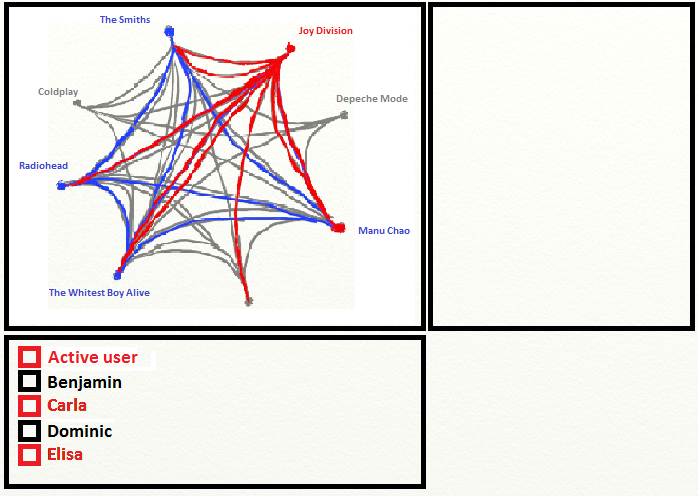
\includegraphics[width=\textwidth]{img/paper_prototype_item_click}
					\caption{Clicking/hovering an item node. When clicking a node, an additional screen would be shown next to the graph. On this screen artist information is displayed.}
					\label{figure:paper_prototype_item_click}
	\end{subfigure}
	\caption{A selection of the screens used in the user study with paper prototype.}%
	\label{figure:paper_prototype}%
\end{figure}

When a user would hover an artist or user name, the screen would be replaced with the corresponding new state of the screen. To ensure a certain degree of freedom, all possible screen states were drawn for the given graph. To keep this amount manageable within the scope of a relatively short user test, the number of artists was limited to eight, and the number of users to six, including the active user. Another reason for keeping graph size small, is that small graphs tend to be easier to interpret\cite{herman:2000}. In an environment where interactions aren't as smooth as in a real implementation, this may be of significance, keeping the principle of transparency\index{principle of transparency} in mind.


\subsubsection{Test parameters}\label{chapter:prototype:section:paper:setup}

Five test users between the ages of $22$ and $26$ were selected. Four of them identified as enthousiasts, one of them as a casual listener. Although they did not necessarily use recommendation systems to actively search for new music, they had a notion of what these systems were.

The focus of the test is on insight, i.e., transparency, and usability, covering satisfaction, learnability and efficiency:

\begin{enumerate}
	\item \textbf{Insight}: Verifying whether or not the user can gain insight into the recommendation rationale.
	\item \textbf{Usability}: Finding out the perceived usability of the application. Discovering usability issues through observation.
\end{enumerate}


%Each task is related to one of those objectives. ELABORATE
The list of tasks that were performed by the users is listed in appendix \ref{appendix:tasklists:prototype1}. The tasks description are based on a template\footnote{A \emph{PDF} version of this template can be found at: \url{http://www.paperprototyping.com/downloads/Ch6_task_template.pdf}} by Carolyn Snyder\cite{snyder:2003}.


\subsubsection{Test results}\label{chapter:prototype:section:paper:results}

% AVG, boxplots / question, boxplot overall

The average SUS score for this iteration was $77$. The distribution of results for each question is shown in figure \ref{fig:iterations_sus_scores_it1_boxplots}. The next paragraphs give a more in-depth analysis of the results.

\begin{figure}
	\begin{center}
		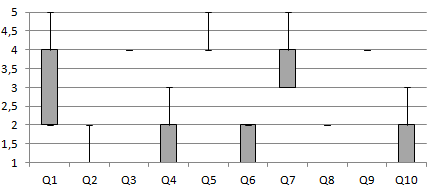
\includegraphics[width=8.3cm]{img/iterations_sus_scores_it1_boxplots}
	\end{center}
	\caption{The SUS results for each question for iteration 1.}
	\label{fig:iterations_sus_scores_it1_boxplots}
\end{figure}


\paragraph{Transparency}

The first part of the test was aimed at forming an initial mental model of the system without interacting with the visualization. When participants were asked to describe what they saw and try to explain the visualization, all of the participants identified the edges as certain relationship between artists. Most of them interpreted the relationship encoded in the edges as a content-based relationship; for example artists that have similar genres are connected.

Blue edges were usually correctly associated with the highlighted active user profile. This insight made one of the users see that the edges represent a co-occurance relationship, i.e., if a user has any set of two items in his/her profile, these items are connected.

If users became aware of the fact that blue nodes and edges corresponded to items that were already owned, item suggestions were easy to point out. In some cases this waited until the second step of the evaluation process where interaction was allowed.

The test users were asked what kind of interactions were possible with the visualization, and what the effects of these actions would be. All of the users listed left mouse clicks. Also dragging and scrolling were suggested by some participants. In that case participants were simply told that this kind of interaction was not supported. They expected to be able to manipulate the edge trajectory by dragging the edges were they wanted. However, clicking an edges is also not supported by the visualization. The effect of clicking a node was usually correctly predicted, although some users did not immediately see that related users would be highlighted as well.

In order to avoid restricting the user to predefined action patterns, the user was relatively free to explore the visualization in the second part of the test. Most participants started by clicking another user's icon and noted the resulting highlights in red in the graph. For one user the tasks in this step were a mere confirmation of the already established mental model. For most users this turned out to be an important moment in adjusting the first model. When alternating between clicking users icons, as well as between artist nodes and artist nodes and user icons the other users were able to correct their model in this step to finally form the correct picture of what the visualization was trying to convey. For two users this took significantly more time than for the other two remaining users.

The understanding of the relationship encoded in the edges, is key to grasping the whole idea behind the visualization. Once this was understood, all users could explain the recommender rationale. Moreover, users were able to point out an item recommendation that was more favourable than another suggestion, illustrating insight at a deeper level. For example using the total number of links to the active user profile, the total amount of related users, or a strong connection with a particular favourite item.


\paragraph{Satisfaction, learnability, and efficiency}

An average SUS score of $77$ suggests that the overal usability is considered to be good - also keeping in mind some of the limitations of paper prototypes. Still, some issues remain: the results for questions \texttt{Q1}, \texttt{Q4}, \texttt{Q7}, and \texttt{Q10} were the lowest. \texttt{Q1} is corresponds to the perceived usefulness, and is related to the overall satisfaction. Scores for \texttt{Q4}, \texttt{Q7}, and \texttt{Q10} may indicate that the learnability of the application can still improve.

Once users were able to develop a strategy for choosing recommendations, they could apply it rather easily in new cases. This suggests that if the user has passed initial learning phase, the system allows for efficient decision making.


\subsubsection{Conclusions}\label{chapter:prototype:section:paper:conclusion}


In conclusion, one user managed to get the complete mental model correct in the first step of the insight gaining process. The others were able to correct it in the second step. The model helped identifying a particular suggestion as more interesting than an others based on what they learned from the visualization.

Table \ref{table:iteration1:issues} gives an overview of the most important issues discovered in this iteration with their priority.

\begin{table}%
	\caption{Overview of the most important issues discovered in the first iteration, using the paper prototype.}
	\begin{center}
		\begin{tabular}{p{70px} | p{180px} | p{180px} }
			\hline
			\textbf{Problem} & \textbf{Priority} & \textbf{Solutions} \\
			\hline
			
			Learnability
			&
			\emph{Medium}: May be due to limitations of the paper prototype. Also, it is expected that a minimal effort is required to learn the system, instead of instantly understanding each aspect of the application.
			& (1) Providing more textual clues, as suggested by test users. (2) Moving towards a digital prototype with the user's actual library as data source. As the user has a better understanding of his/her own music library, it is likely that relationships within this data can be discovered more rapidly. % increased domain relevance
			\\
			
			Satisfaction
			&
			\emph{Medium}: Low value of usefulness may be due to the fact that the data is not personalized. The recommendations were also not based on an actual case, but were selected in the hope to appeal to the majority of test users.
			&
			(1) Again, moving towards real, personalized data may improve this aspect of the prototype.
			\\
			
			\hline
		\end{tabular}
	\end{center}
\label{table:iteration1:issues}
\end{table}

% In terms of the usability characteristics, the prototype ...

% terugkoppelen naar usability properties: learnability, Error rate and severity, Efficiency, Satisfaction, Memorability (see future user tests)
% does the explanation system provide transparency?
% can users gain insight into the visualization?




%%%%%%%% ITERATION 2
\subsection{Iteration 2: first digital prototype (SoundSuggest 1.x)}\label{chapter:prototype:section:soundsuggest1}

\subsubsection{The prototype}\label{chapter:prototype:section:soundsuggest1:prototype}

% changes from previous iteration
As the test users were able to discover the recommender rationale using the visualization, and no notable usability issues had arisen, we started working on the digital prototype. This prototype used static data, but already supported all the use cases listed in appendix \ref{appendix:use_cases}. The resulting prototype can be seen in figure \ref{figure:prototype_soundsuggest1}.


% iteration 2 : prototype
\begin{figure}
	\centering
	\begin{subfigure}[t]{0.3\textwidth}
					\centering
					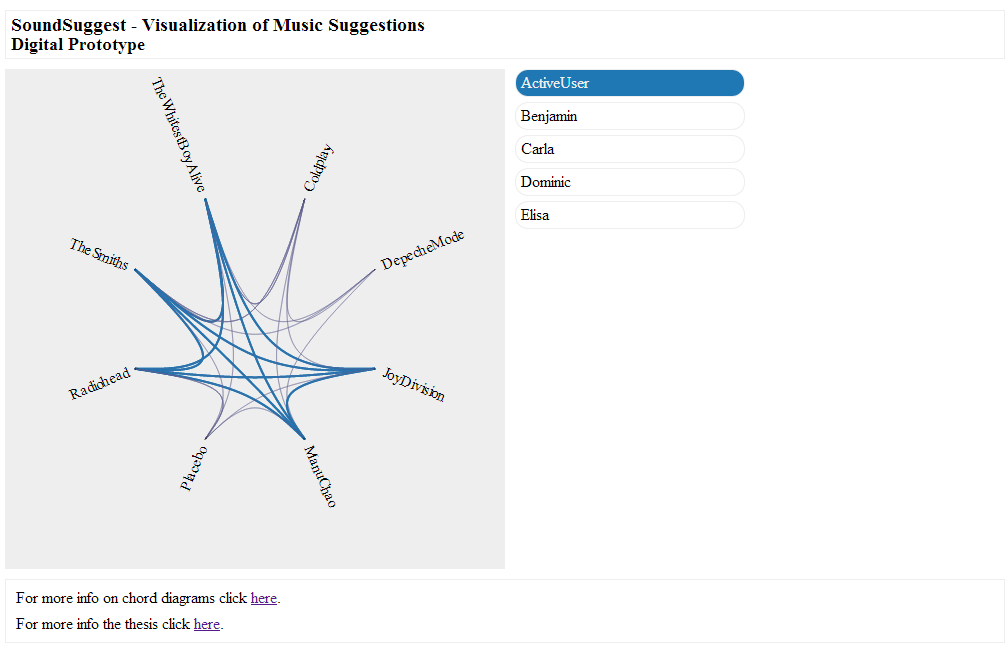
\includegraphics[width=\textwidth]{img/prototype_soundsuggest1_default}
					\caption{The default visualization with the active users items highlighted.}
					\label{figure:prototype_soundsuggest1_default}
	\end{subfigure}%
	~
	\begin{subfigure}[t]{0.3\textwidth}
					\centering
					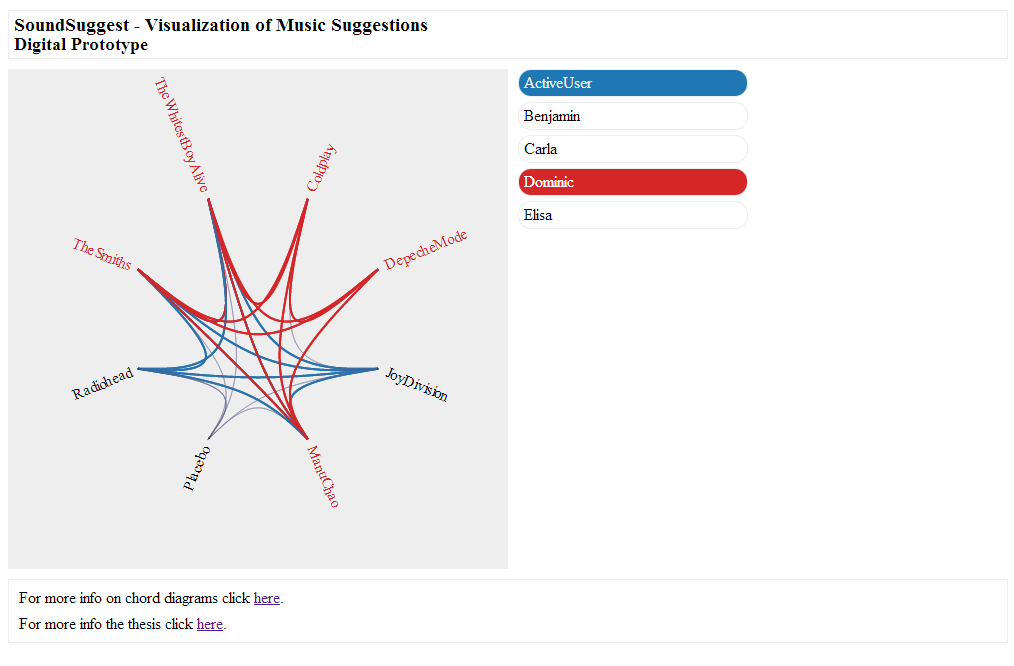
\includegraphics[width=\textwidth]{img/prototype_soundsuggest1_user_click}
					\caption{Clicking a user list element.}
					\label{figure:prototype_soundsuggest1_user_click}
	\end{subfigure}
	~
	\begin{subfigure}[t]{0.3\textwidth}
					\centering
					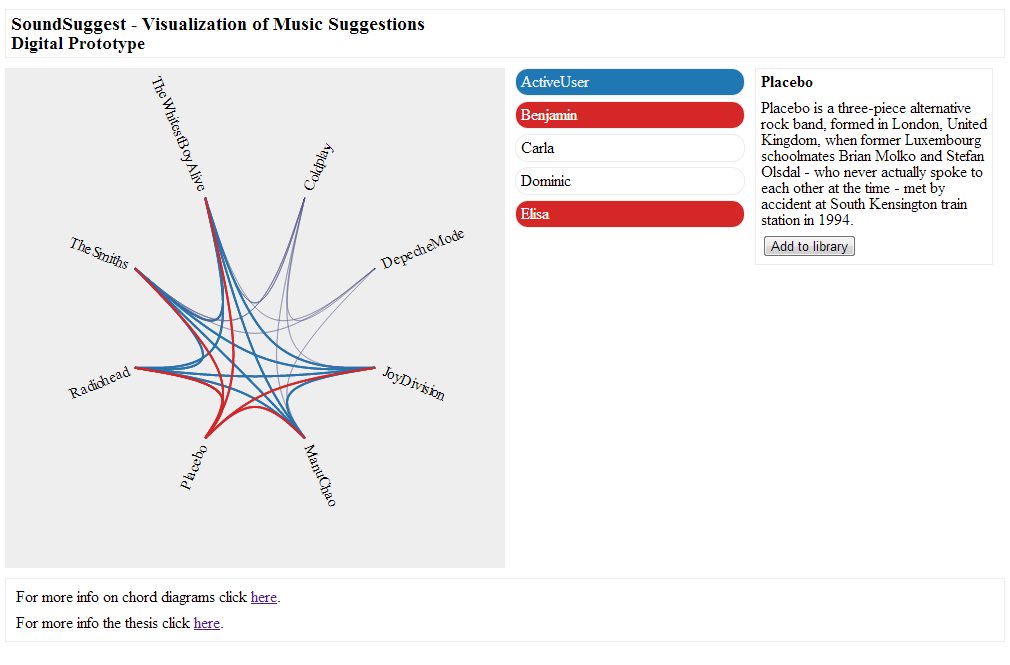
\includegraphics[width=\textwidth]{img/prototype_soundsuggest1_item_click}
					\caption{Clicking an item node.}
					\label{figure:prototype_soundsuggest1_item_click}
	\end{subfigure}
	\caption{A selection of the screens used in the user study with the first digital prototype.}%
	\label{figure:prototype_soundsuggest1}%
\end{figure}



\subsubsection{Test parameters}\label{chapter:prototype:section:soundsuggest1:setup}

Test users were selected in a similar manner as in the first iteration. Two test users from the previous iteration were tested again, the other three were new test users. The test users that had been tested before, were tested first. Memorability was evaluated for these subjects along with the other objectives for this iteration. Based on listening habits, one savant, two enthousiasts and two casual listeners were tested.

The objective are the same as in iteration one. However, in addition to these objectives we want to find out how successful the transformation from paper to digital prototype had been. Also feedback was asked on a help file that was made for the application.

The tasks remained the same as in the previous iteration. The test users that were tested in the first iteration also were asked if there were any improvements or new issues going from the paper prototype to a digital one. Remarks made by these persons were also presented to the other test users.


\subsubsection{Test results}\label{chapter:prototype:section:soundsuggest1:results}

The average SUS score for this iteration was $79.5$. The distribution of results for each question is shown in figure \ref{fig:iterations_sus_scores_it2_boxplots}. A detailed analysis of the results is given in the following paragraphs.

\begin{figure}
	\begin{center}
		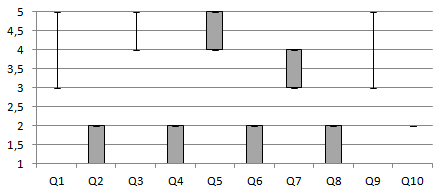
\includegraphics[width=8.3cm]{img/iterations_sus_scores_it2_boxplots}
	\end{center}
	\caption{The SUS results for each question for iteration 2.}
	\label{fig:iterations_sus_scores_it2_boxplots}
\end{figure}

\paragraph{Transparency}

Test users listed the list of neighbours, artist names. Most of them also noted that certain items and edges were coloured blue. One user also immediately saw that some of the other users and items did not have this colour and explained that these items corresponded to items recommended by these users. This participant further clarified that he expected that for each neighbour a similar coloured structure would exist as for the highlighted active user. When asked how this helped him understanding the recommendation rationale, the test user explained that these were users that had similar tastes as the active user. Items in these profiles were then candidate recommendations.

The other users did not find the recommendation rationale in the first step. When interacting with visualization however, they were able to tell similar stories. Again, the key to understanding the visualization turns out to be understanding what contextual information is that is encoded in the link between artist nodes. For most users this could be discovered by comparing the neighbour profile with the active user's profile on the graph.

With regard to the first iteration, one particular difficulty was mentioned by both users that tested the paper prototype: in the paper prototype parallel edges were easy to discern, but in the edge-bundling algorithm used, parallel edges will overlap in the resulting visualization. This makes it harder to see the connection between a clicked artist, and the number of neighbours that were highlighted. However, when the new test users were asked if they saw this as a problem, they acknowledged that this could help, but didn't see it as a major improvement. An improvement in the digital prototype was that the smoothness of interactions had of course greatly increased, which made it much easier to compare items and users, according to the test users.

% ---> no surprise that neighbour clicked --> insight, artist click ---> not so much

When asked to add one of the recommendations to the active user profile, all users could give one or more reasons, similar to the first iteration.


\paragraph{Satisfaction, learnability, memorability, and efficiency}

Some usability issues surfaced during the think aloud test. Two users thought that deselecting an item or user should be triggered by clicking somewhere outside the graph as well. Some test users complained that the help files did not have a table of contents or some sort of overview. Two users stated that it would be nice to have some kind of overview of the meaning behind each colour. Also having an extra colour to distinguish between selected profiles or edges and hover queries would be a welcome addition.

Overall, the SUS questionnaire results stayed more or less stable. Results for question \texttt{Q7} are still rather low, indicating that users still don't see the system as very easy to learn.

In terms of efficiency the same idea as in iteration $1$ applies. Of course, as interactions are much faster, this also has a positive effect on the efficiency of system usage.


\subsubsection{Conclusions}\label{chapter:prototype:section:soundsuggest1:conclusion}

% parallel edge occlusion: previously tested users say it would help, especially to see when two users share a parallel edge - otherwise hard to see which users have what items if overlap, but it is still clear.
% also, new test users were able to still get the recommender rationale

Overall, the transition from paper to digital prototype was successful, apart from the issue with parallel edges overlapping. Although it would be interesting if this problem could be solved, users indicated that was not a particular barrier for gaining insight into the recommendation rationale.

Different colours for hovering and selecting, although others thought this wasn't really necessary. Users suggested to add an option to choose between different encodings with an additional legend for the meaning of the different colours. Also options to alter the number of items shown were considered useful additions to the application's functionality.

Table \ref{table:iteration2:issues} gives an overview of the most important issues for iteration 2.

\begin{table}
	\caption{Overview of the most important issues discovered in the second iteration, using the first digital prototype.}
	\begin{center}
		\begin{tabular}{p{70px} | p{180px} | p{180px} }
			\hline
			\textbf{Problem} & \textbf{Priority} & \textbf{Solutions} \\
			\hline
			
			Parallel edges overlap
			&
			\emph{Low}: If possible, it would be nice to see this problem solved, but it is not considered to be a priority.
			&
			(1) Developing a new graph drawing algoritm, although this is perhaps beyond the scope of this thesis. (2) Allowing to change the bundling strength might improve the overall layout of the graph.
			\\
			
			Meaning behind colour encodings.
			&
			\emph{High}: As there already is a significant amount of implicit information in the visualization, it may be wise to give some direct clues as well.
			&
			(1) Show a legend of the visual encodings. (2) Enable the user to choose encodings him/herself. % see Ware: beware to not make this too complicated
			\\
			
			Deslecting an item
			&
			\emph{Medium}: Most users did not really had a problem with this, but it seems this could be solved easily enough.
			&
			(1) Adding a button to clear the current selection. (2) Track click events outside the visualization to clear the selection.
			\\
			
			\hline
		\end{tabular}
	\end{center}
\label{table:iteration2:issues}
\end{table}



%%%%%%% ITERATION 5
\subsection{Iteration 3: second digital prototype (SoundSuggest 2.x)}\label{chapter:prototype:section:soundsuggest2}

\subsubsection{The prototype}\label{chapter:prototype:section:soundsuggest2:prototype}

% changes from previous iteration
The layout from the previous iteration was retained, but this time the visualization was incorporated into a chrome suggestion that could be injected directly into the \emph{Last.fm} recommendations page, using real data.

An option menu was added with options to alter the data settings, and colour encodings. Data settings that could be answered were the number of recommendations shown, the number of top artists from the active user's profile shown, and the number of neighbours included in the visualization. Another option was to change the threshold. The threshold corresponds to the clustering range of the data collection algorithm. A low threshold value will allow the user to have a link to a certain artist without owning it. Instead the user may own one or more related artists, i.e., the neighbour is required to have a link to an item inside a cluster of items, rather than a particular item. The settings menu is shown in figure \ref{figure:prototype_soundsuggest2_settings}.

\begin{figure}%
	\begin{center}
		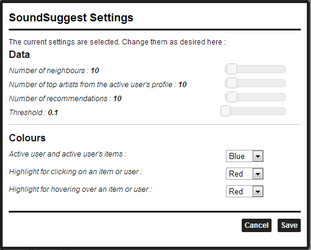
\includegraphics[width=200px]{img/prototype_soundsuggest2_settings}%
	\end{center}
	\caption{The settings menu of the second digital prototype.}%
	\label{figure:prototype_soundsuggest2_settings}%
\end{figure}


To solve the problem of deselecting an item, an additional button titled \emph{Clear selection} was added in the menu bar. As the data loads, a spinner indicates to the user that the system is busy, as can be seen in figure \ref{figure:prototype_soundsuggest2_loading_data}. The resulting prototype is shown in figure \ref{figure:prototype_soundsuggest2}.

\begin{figure}%
	\begin{center}
		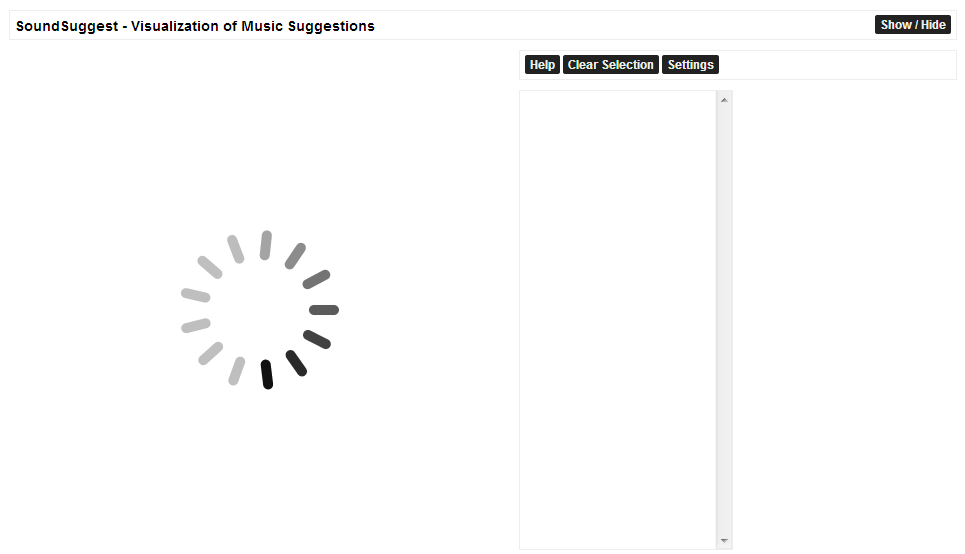
\includegraphics[width=200px]{img/prototype_soundsuggest2_loading_data}%
	\end{center}
	\caption{When the data is loading, a spinner is shown to indicate something is happening.}%
	\label{figure:prototype_soundsuggest2_loading_data}%
\end{figure}


% ITERATION 3
\begin{figure}
	\centering
	\begin{subfigure}[t]{0.3\textwidth}
					\centering
					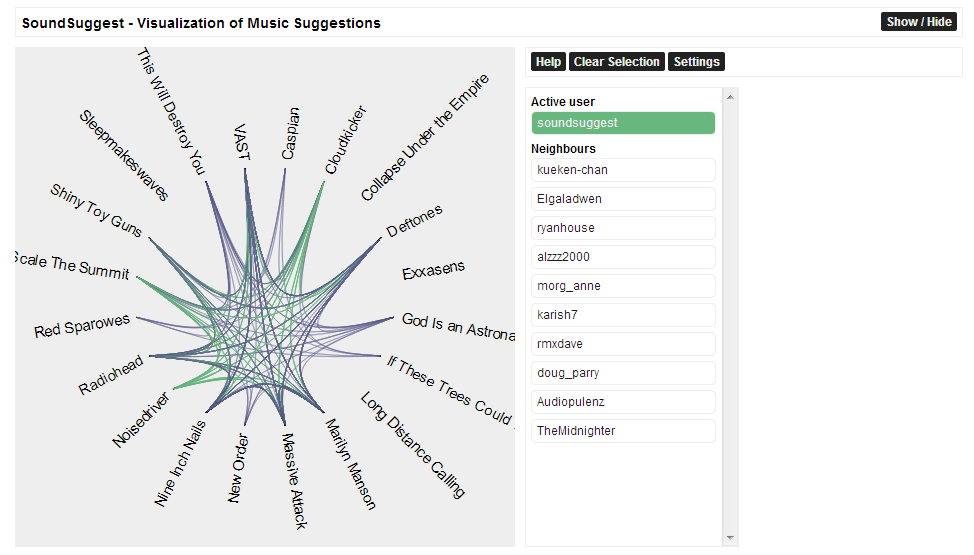
\includegraphics[width=\textwidth]{img/prototype_soundsuggest2_default}
					\caption{The default visualization with the active user's items highlighted.}
					\label{figure:prototype_soundsuggest2_default}
	\end{subfigure}%
	~
	\begin{subfigure}[t]{0.3\textwidth}
					\centering
					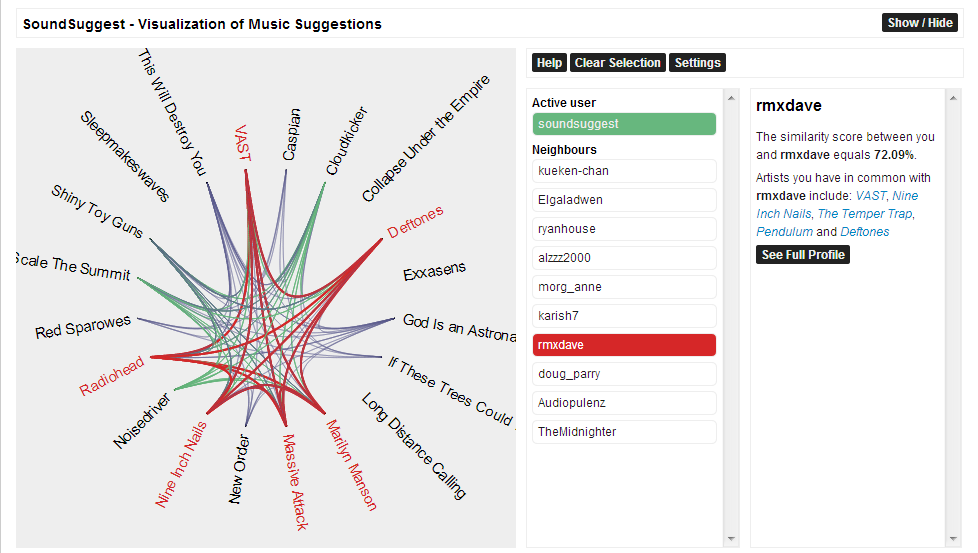
\includegraphics[width=\textwidth]{img/prototype_soundsuggest2_user_click}
					\caption{Clicking a user list element.}
					\label{figure:prototype_soundsuggest2_user_click}
	\end{subfigure}
	~
	\begin{subfigure}[t]{0.3\textwidth}
					\centering
					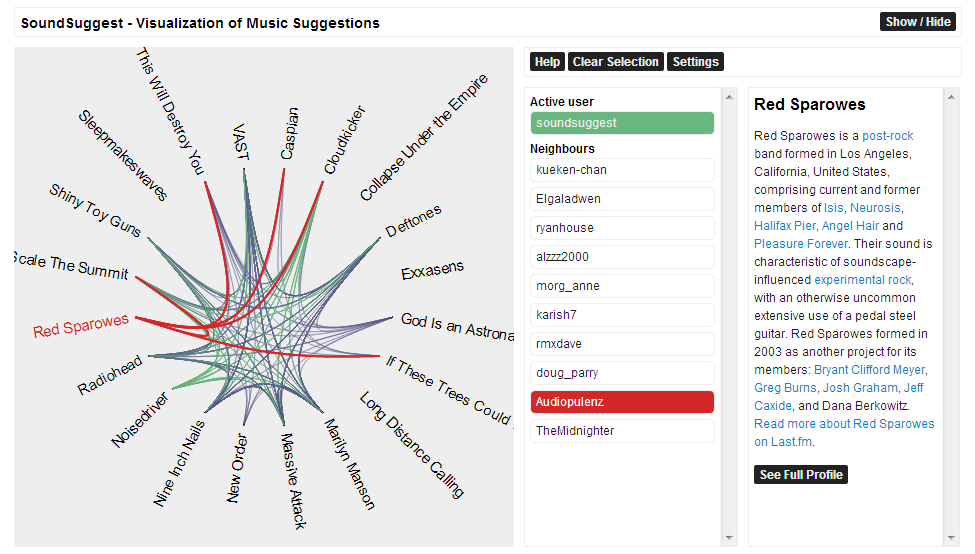
\includegraphics[width=\textwidth]{img/prototype_soundsuggest2_item_click}
					\caption{Clicking an item node.}
					\label{figure:prototype_soundsuggest2_item_click}
	\end{subfigure}
	\caption{A selection of the screens used in the user study with the third digital prototype.}%
	\label{figure:prototype_soundsuggest2}%
\end{figure}



\subsubsection{Test parameters}\label{chapter:prototype:section:soundsuggest2:setup}

Five test subjects were selected, who were \emph{Last.fm} users between the ages of $22$ and $26$. Three of them used the website or its \emph{Scrobbler} on a weekly basis or even more frequently, the other two only used \emph{Last.fm} on a monthly basis. Two users had tested both the paper and first digital prototype, one other user already had tested the paper prototype.

The objectives of the test remained the same. In addition to the previous objectives the performance of the application was investigated as well. Concerning usability, there were three areas of interest:

\begin{enumerate}
	\item \textbf{Visualization}: The general usability of the visualization according to new users.
	\item \textbf{Option menu}: General usability of the options menu.
	\item \textbf{Chrome extension}: The placement of the application into the \emph{Last.fm} recommendations page.
\end{enumerate}

The tasks listed in appendix \ref{appendix:tasklists:prototype2} were used to investigate these areas. Insight by new users could again be tested using the scheme in appendix \ref{appendix:tasklists:prototype1}. To get an idea of the learnablity and memorability of the application, test users from previous iterations were asked to explain the visualization rationale again before the rest of the test.


\subsubsection{Test results}\label{chapter:prototype:section:soundsuggest2:results}

The average SUS score for this iteration was $76.5$. The distribution of results for each question is shown in figure \ref{fig:iterations_sus_scores_it3_boxplots}.

\begin{figure}
	\begin{center}
		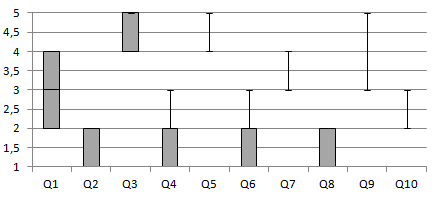
\includegraphics[width=8.3cm]{img/iterations_sus_scores_it3_boxplots}
	\end{center}
	\caption{The SUS results for each question for iteration 3.}
	\label{fig:iterations_sus_scores_it3_boxplots}
\end{figure}


\paragraph{Transparency and memorability}

Users from previous iterations were able to recall the visualization rationale from previous sessions, although two of them needed to interact with the visualization before they could remember it accurately. This suggests that the memorability of the explanation system is adequate. Based on previous experience and insight, one of these users explained he had found a new reasoning to select an artist based on the graph.

When testing insight for new users, no notable differences from previous iterations occurred. Theey also needed interaction with the visualization before the recommender rationale could be discovered.


\paragraph{Usability, satisfaction, efficiency, and learnability}

The settings menu was found by all users when asked to change the number of visualized items and/or users. One of the remarks when changing the data settings, was that the visualization would take long to load. As there were now more edges and nodes, some scalability issues came into play: some users complained that the increased number of edges would create clutter that made it hard to compare profiles.

Another issue that was mentioned was that it was hard to distinguish between recommendations once the test user started hovering over the listed neighbours. A test user from the previous session noted that this was less of a concern in the previous prototype, as the number of nodes was much lower.

The threshold option turned out to be very confusing, even with an explanation from the help files. Also, the results of changing the threshold were not visually pleasing either. As soon as the threshold would be over $0.1$, the connectivity dropped and some edges that were previously connected were no longer connected. This may also explain the fact that the average SUS score is lower than in previous iterations.

When adding a recommendation to the user profile, to see the changes in the profile, the whole page needed to be refreshed instead of just the visualization. Also, if the user would refresh or navigate away from the page, all of the data would have to be reloaded. This also has a negative effect on the satisfaction of system usage, which may also provide an additional explanation for the lower overal score.



\subsubsection{Conclusions}\label{chapter:prototype:section:soundsuggest2:conclusion}

Apart from the threshold option, the settings menu posed no notable difficulties. It would probably be better to use a default setting for the threshold, and remove the option from the settings menu altogether. The other options can remain as they are.

In conclusion, the main issues from the previous iteration have been solved. Table \ref{table:iteration3:issues} gives an overview of the most important issues for iteration $3$.

\begin{table}
	\caption{Overview of the most important issues discovered in the third iteration, using the second digital prototype.}
	\begin{center}
		\begin{tabular}{p{70px} | p{180px} | p{180px} }
			\hline
			\textbf{Problem} & \textbf{Priority} & \textbf{Solutions} \\
			\hline
			
			Threshold
			&
			\emph{High}: It is confusing and clearly has a negative impact on the overal user experience.
			&
			(1) Remove this functionality.
			\\
			
			Data load speed
			&
			\emph{High}: The main problem lies with the fact that changing the settings, reloading the page, and so on, results in reloading all the data, even though all the required data is known.
			&
			(1) Simply keeping a local copy of the latest version of the data. This version can then be updated either manually, or by checking for updates over a predefined time interval.
			\\
			
			Visual clutter
			&
			\emph{High}: Becomes an important problem as the graph size increases. May hinder the insight gaining process. May prohibit users from efficiently comparing user profiles and recommendations.
			&
			(1) Changing the graph layout: clustering nodes, changing edge-bundling strength, allowing to move nodes. (2) Change edge opacity to avoid visual clutter within dense regions of the graph. (3) Selectively hide elements temporary.
			\\
			
			\hline
		\end{tabular}
	\end{center}
\label{table:iteration3:issues}
\end{table}




%%%%%%% ITERATION 4
\subsection{Iteration 4: third digital prototype (SoundSuggest 3.x)}\label{chapter:prototype:section:soundsuggest3}

\subsubsection{The prototype}\label{chapter:prototype:section:soundsuggest3:prototype}

% changes from previous iteration

To reduce issues with distinguishability, an additional option was added to the settings menu to alter the \emph{tension} of the edges, i.e., the edge-bundling strength. This way, the user would be able to alter the layout to a certain extend.

To make it easier to distinguish between recommendations and top artists, the node labels for top artists are underlined in the graph.

A button to refresh the data and update the visualization was added to solve the problem of having to refresh the whole page to have the latest version of the data.

To avoid long waiting times when loading the page, the data that was loaded last was cashed. This way the latest data set could be loaded quickly from local storage. The refresh button can be used to get an up-to-date version of the data.

An example of the resulting visualization is shown in figure \ref{figure:prototype_soundsuggest3}.

% ITERATION 4
\begin{figure}
	\centering
	\begin{subfigure}[t]{0.3\textwidth}
					\centering
					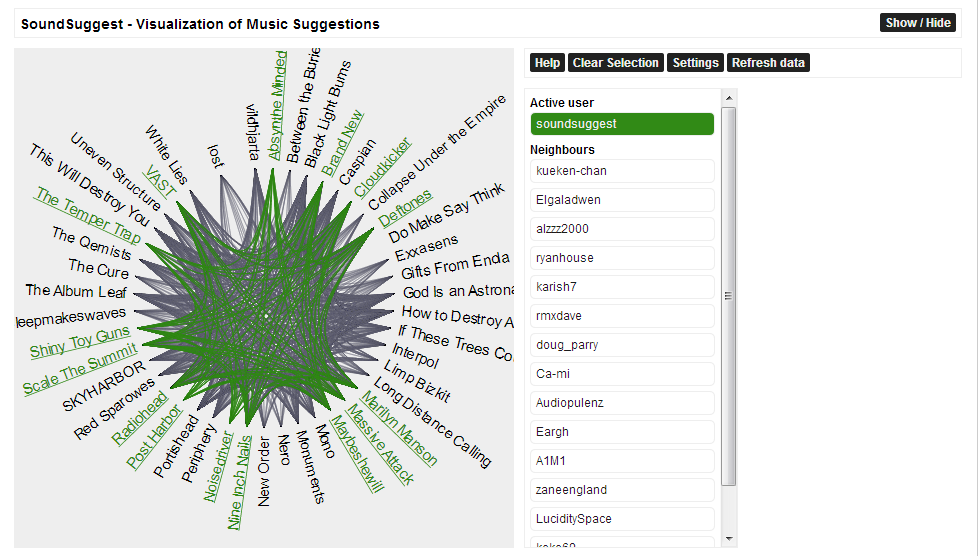
\includegraphics[width=\textwidth]{img/prototype_soundsuggest3_default}
					\caption{The default visualization with the active user's items highlighted.}
					\label{figure:prototype_soundsuggest3_default}
	\end{subfigure}%
	~
	\begin{subfigure}[t]{0.3\textwidth}
					\centering
					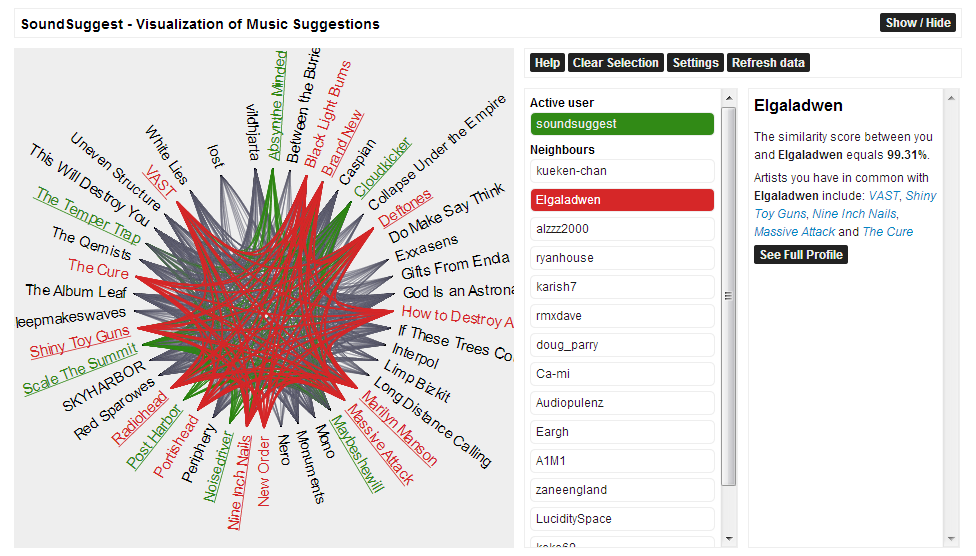
\includegraphics[width=\textwidth]{img/prototype_soundsuggest3_user_click}
					\caption{Clicking a user list element.}
					\label{figure:prototype_soundsuggest3_user_click}
	\end{subfigure}
	~
	\begin{subfigure}[t]{0.3\textwidth}
					\centering
					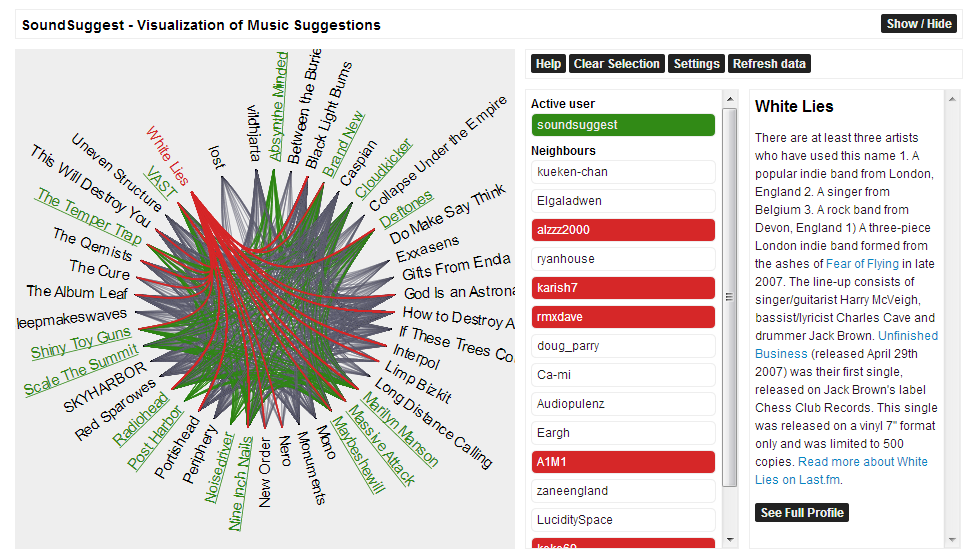
\includegraphics[width=\textwidth]{img/prototype_soundsuggest3_item_click}
					\caption{Clicking an item node.}
					\label{figure:prototype_soundsuggest3_item_click}
	\end{subfigure}
	\caption{A selection of the screens used in the user study with the third digital prototype.}%
	\label{figure:prototype_soundsuggest3}%
\end{figure}



\subsubsection{Test parameters}\label{chapter:prototype:section:soundsuggest3:setup}

Ten test users were selected. Three of these users already had experience with the application based on the previous iteration. Two of the other test users had tested one the first digital prototype. The other test users were new users. All of the test users had some experience with Last.fm or other music recommenders like \emph{Grooveshark}, \emph{Spotify} or \emph{Youtube}. If users didn't have a Last.fm account, they were asked to create one one to two weeks in advance and add their listening habits to their Last.fm profile.

% users: show diagrams with distribution for listening habits, Last.fm usage

For new users insight could again be tested using the tasks in appendix \ref{appendix:tasklists:prototype1}. The tasks listed in appendix \ref{appendix:tasklists:prototype3} were used to test the following explanation system properties: \emph{transparency}, \emph{effectiveness}, \emph{persuasion}, \emph{trust}, and \emph{satisfaction}.

Although \emph{scrutanability}\index{scrutanability} could have been tested by removing undesired recommendations from the list under the visualization, the visualization did not seem to include this information immediately when refreshing the data. It is also not really clear to what extend the information of removed suggestions is included into future recommendations by Last.fm's recommender algorithm.

% Efficiency is not explicitly tested here. For example benchmark tasks ... perceived effeiciency ...  rely on usability


\subsubsection{Test results}\label{chapter:prototype:section:soundsuggest3:results}

The average SUS score for this iteration was $80.5$. The distribution of results for each question is shown in figure \ref{fig:iterations_sus_scores_it4_boxplots}.

\begin{figure}
	\begin{center}
		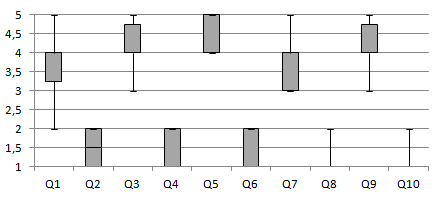
\includegraphics[width=8.3cm]{img/iterations_sus_scores_it4_boxplots}
	\end{center}
	\caption{The SUS results for each question for iteration 4.}
	\label{fig:iterations_sus_scores_it4_boxplots}
\end{figure}


\paragraph{Transparency}

All of the test users were able to describe the recommendation rationale. Most of them used a variation on the following: \textit{Last.fm looks for users that have a similar taste, based on the active user's favourite artists, i.e., neighbours. Last.fm decides which items owned by these neighbours are interesting for recommendation based on preference by neighbours, i.e., top artists in the neighbouring profiles, and the total number neighbours that own these items}.


\paragraph{Trust, effectiveness, and persuasion}

Most users already knew more or less who the recommended artists were. For some users this would increase trust, as they basically forgot about them when building up listening history. For other users this would actually decrease their trust in the system as they just were not interested in the recommendation. Interestingly Last.fm's own explanation for recommending the item was usually displeasing. Last.fm would justify the recommendation by listing a number of 'similar' artists. Unfortunately, for some categories of artists there exists some bias in the recommendations. For example musicians that have a solo project and also played in a series of different bands lets Last.fm consider these artists as similar. Another example is that artist recommendations for bands and musicians that operate in a country with a less international music scene would be influenced by regional effects. Belgian bands would be considered similar just for beging Belgian to the point were all similar artist pages on the \emph{Last.fm} website would be Belgian regardless of their genre. Users confirmed that this kind of bias reduces the trust in the recommender system. On the other hand, it was interesting to see that this bias could actually be detected in the visualization as neighbours usually did not have edges going from items in their profile to these 'biased' recommendations.

When users did not know a certain recommendation, most users were interested if the recommendation occurred in one of the neighbouring profiles. In this sense the visualization helped persuade the users check out certain artists. From the six users that checked out an item they did not already know, four of them found at least one item that they liked and added to their profile. When discovering a new item that they liked, users admitted this significantly increased their trust in the recommender system, even more than when they found an item that they liked but already knew about.

Although the explanation system was not always as effective in helping to find good recommendations, it provided an additional means for the user to establish his/her own approach for finding recommendations. For example a user would look at neighbours for artist suggestions, rather than just the artist recommendations by \emph{Last.fm}.



\paragraph{Satisfaction, memorability, learnability, and efficiency}

The fact that the data set was cashed made users much more confident in clicking links, as they didn't had to worry about long loading times.

A problem that remained was the scalability of the graph. When visualizing a total of over $40$ recommendations and top artists, loading times not only increase but the density caused by overlapping edges, makes it hard to compare user profiles. Although the tension parameter was visually pleasing, this did not completely resolve these scalability issues. Most users liked a tension in the area of $0.45$ to $0.60$ for graphs including up to $40$ nodes. Beyond this amount of nodes its effects became less important.

By underlining owned artists, it had become easier to compare user profiles. Users from previous iterations stated that this was definitively an improvement, but that there might still be better ways to visualize this. % still room for improvement

The distribution of scores for each separate SUS question for the last iteration is shown in figure \ref{fig:iterations_sus_scores_it4_boxplots}. The questions with the lowest scores were the first question and the seventh question. It should be noted thaht all test users were frequent \emph{Last.fm} users and also not all of the test users used the Chrome browser that was required for running the Chrome extension. Nonetheless there were test users that were very positive about the application in that respect as well. Although there were no negative votes for question 7, a lot of users were not convinced that using the application was easy to learn. There might still be some work left to make the application more accessible to casual users.




%The refresh button proved useful when adding a new recommendation.

% 1. Find three neighbours that are closely related to you, based on the visualization.
% 2. Find three recommended artists you think are interesting.
% 3. Explain the recommendation rationale (transparency).
% 4. Find a suggestion for an artist you didn't know about.
%		Would you like to check our this artist's profile and listen one or more songs by this artist (persuasion)?
%		Do you think the recommender system has made a good suggestion? Would you add it your profile (effectiveness)?
%		How does it affect your trust in the recommender system (trust)?





% risk pays of if the result is good!!


\subsubsection{Conclusions}\label{chapter:prototype:section:soundsuggest3:conclusion}

One issue that was resolved between the user tests was that the artist names that were used to create CSS \texttt{id} and \texttt{class} names sometimes contained special characters causing the visualization to not function correctly anymore. This was solved by using the hash value of the artist name instead. Although no new iteration was started for this alteration, this may have influenced some of the test results. Overall this only affected two participants.

Based from the choice of the tension parameter by users, a better default value for the tension setting would probably be around $0.55$.

%In future iterations the problems with overlapping edges should be addressed, for example by decreasing the alpha value of egdes that are not relevant to the selection. This is one of the clutter reduction techniques described in \cite{ellis:2007}.

%As trust increases 

Overall, the application scores well based on the user's feedback. It enables users to discover some characteristics of \emph{Last.fm}'s recommender.

Figure \ref{fig:iterations_sus_scores_boxplots} shows the evolution of the SUS values over the four iterations. Based on the percentile rank, the average score of $80.5$ for the final iteration procudes a grade of \texttt{A}.

\begin{figure}
	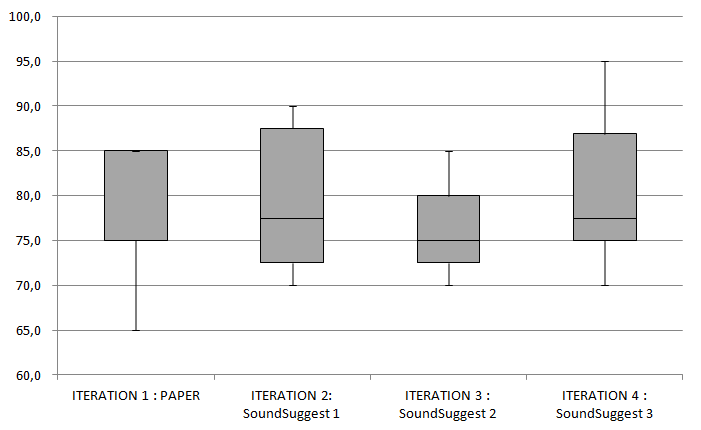
\includegraphics[width=8.3cm]{img/iterations_sus_scores_boxplots}
	\caption{The evolution of the SUS values over the four iterations, visualized as box plots.}
	\label{fig:iterations_sus_scores_boxplots}
\end{figure}



Table \ref{table:iteration4:issues} gives an overview of the most important issues for iteration $4$.

\begin{table}
	\caption{Overview of the most important issues discovered in the fourth iteration, using the third digital prototype.}
	\begin{center}
		\begin{tabular}{p{70px} | p{180px} | p{180px} }
			\hline
			\textbf{Problem} & \textbf{Priority} & \textbf{Solutions} \\
			\hline
			
			Clutter reduction in dense graphs
			&
			\emph{High}: Visual clutter may hinder the insight gaining process, and may prohibit the user of comparing recommendations and user profiles effectively.
			&
			(1) Sorting the artists by recommendation or top artist would make it even easier to distinguish between owned and recommended artists. (2) Clutter reduction through change in opacity between elements that are relevant and irrelevant to the selection. (3) Selectively hiding users and their corresponding edges in the graph.
			\\
			
			Data load efficiency
			&
			\emph{Medium}: Some initial load of data will always be necessary, so for evaluation purposes this is probably a lesser concern.  To target a larger audience, this will become increasinly important.
			&
			(1) Using another algorithm that focuses less on node connectivity, but more on the quantity of data. When more items are involved, connectivity within the graph is likely to be higher as well. (2) Updating the graph as more data loads, depending on the predefined settings. (3) When refreshing the data, only update items that are new.
			\\
			
			Learnability
			&
			\emph{Medium}: Although the functionality of the application seems to be easy enough to learn, e.g. using the options in the settings menu, learning how the application can be useful, still takes up some time. This is probably reflected by lower scores for questions \texttt{Q1}, \texttt{Q7}, and \texttt{Q3}.
			&
			(1) Further refining labels and other visual clues for the end user.
			\\
			
			\hline
		\end{tabular}
	\end{center}
\label{table:iteration4:issues}
\end{table}
